\begin{figure}
\begin{subfigure}{\columnwidth}
  \centering
  %\vspace{-10pt}
  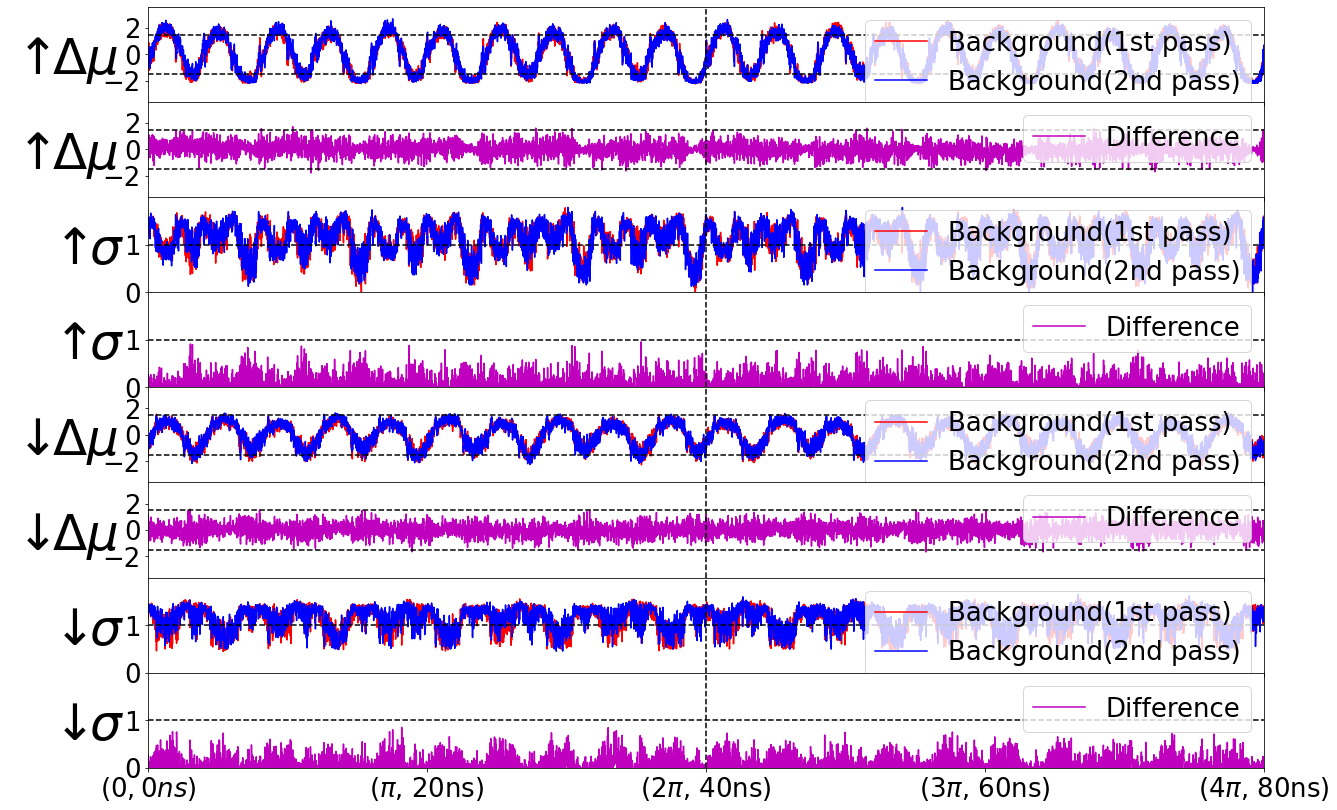
\includegraphics[width=\linewidth,height=5.2cm]{img/base_DIFF_aws_std_ham_pn_4pi.png}
 % \vspace{-15pt}
  \caption{AWS Sensor Only }
  \label{fig:phi-aws-base}
\end{subfigure}
\bigskip
\centering
\begin{subfigure}{\columnwidth}
  \centering
  %\vspace{-10pt}
  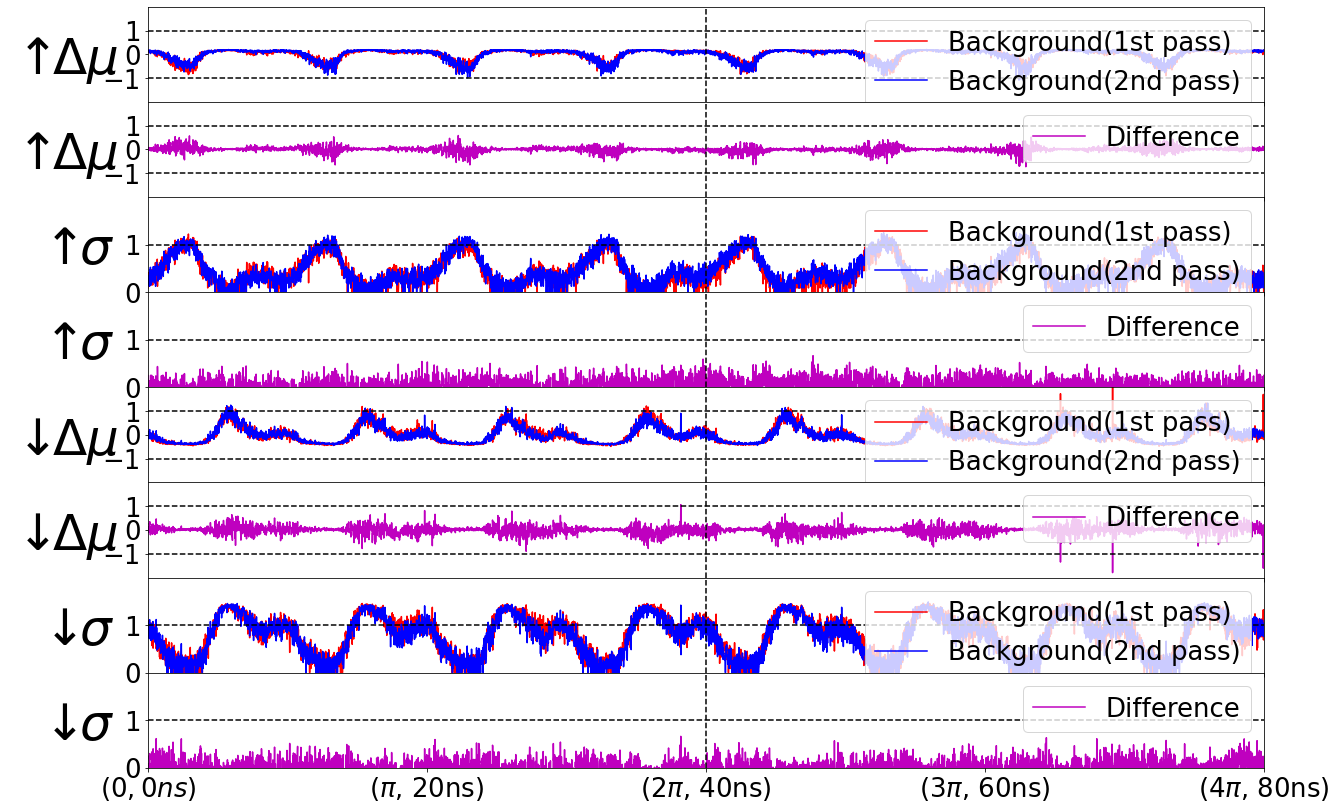
\includegraphics[width=\linewidth,height=5.2cm]{img/base_DIFF_pynq_std_ham_pn_4pi.png}
  %\vspace{-15pt}
  \caption{PYNQ-Z2 Sensor Only}
%  \caption{Baseline (Falling Transition)}
  \label{fig:phi-pynq-base}
\end{subfigure}
\bigskip
\centering
\begin{subfigure}{\columnwidth}
  \centering
  %\vspace{-10pt}
  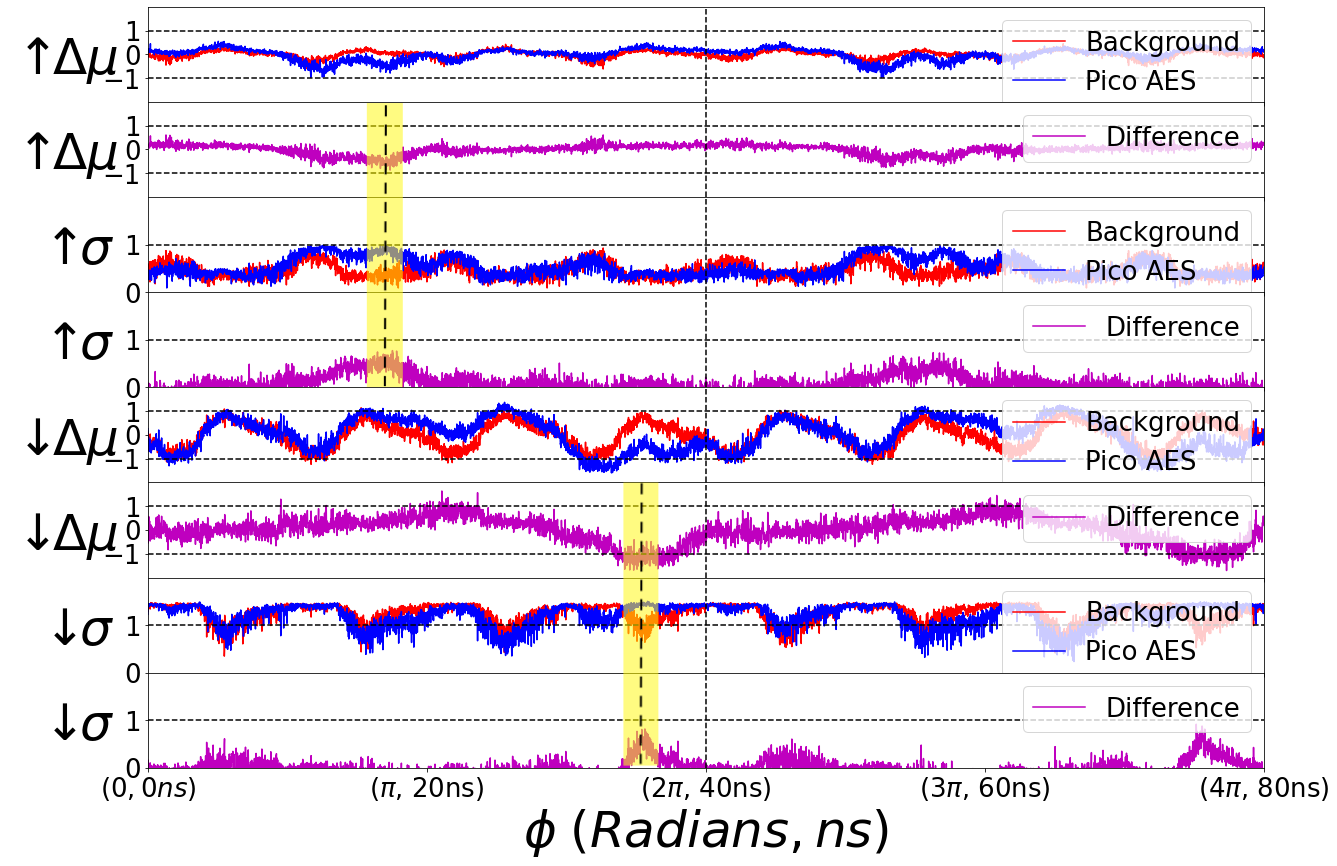
\includegraphics[width=\linewidth,height=5.2cm]{img/pico_aes_DIFF_pynq_std_ham_pn_4pi.png}
  %\vspace{-15pt}
  \caption{PYNQ-Z2 PicoRV AES}
%  \caption{Baseline (Falling Transition)}
  \label{fig:phi-pynq-pico}
\end{subfigure}
\bigskip
\centering
%\vspace{-25pt}
\caption{Measuring sensor output as $\phi$ is swept from 0 to 4$\pi$ on AWS and PYNQ. Background subtraction is necessary to isolate a target from other information sources on the system and reveal the value of $\phi$ where the side channel between the target and the sensor is maximized.}
%\vspace{-15pt}

\label{fig:phi-diff}

\end{figure} 
